Recent years have witnessed a resurgence in partisan polarization in the United States. Politically engaged citizens hold more diverging policy
views, are more ideologically extreme, and exhibit stronger negative affect towards out-partisans than in the past \citep{hetherington2001resurgent, abramowitz2008polarization, iyengar2012affect, mason2014disrespectfully, huddy2015expressive, iyengar2015fear}. A growing literature in moral psychology attributes this divide (at least partially) to fundamental differences in moral frameworks that guide liberal and conservative thinking \citep[e.g.,][]{haidt2012righteous,graham2013moral}. A recent analysis by \citet{garrett2018moral}, for example, finds that individual tendencies to moralize politics exacerbates affective polarization between Democrats and Republicans, which ultimately results in greater social distance and hostility towards out-partisans. More generally, moral conviction as an attribute of attitude strength has been shown to have wide-ranging behavioral consequences \citep{skitka2005moral,skitka2014social}, including diminishing people's willingness to compromise in the realm of politics \citep{ryan2014reconsidering,ryan2017no}.

Do these findings imply that morality in politics is always bound to foster disagreements and hostility between opposing views? Recent research building on Moral Foundations Theory pioneered by \citet{haidt2007new} and colleagues suggests otherwise. According to this view, disagreements about morality are rooted in the underlying intuitions that form people's moral frameworks \citep{haidt2012righteous}. For instance, differential emphasis on basic moral dimensions predicts attitudes on culturally divisive issues such as abortion, the death penalty, or same-sex marriage \citep{koleva2012tracing}. More importantly, however, speaking the same ``moral language'' can overcome ideological divides. Indeed, political arguments can persuade individuals holding opposing views to the extent that they are emphasizing common moral ground \citep[e.g.,][]{day2014shifting,feinberg2015gulf}. Moral frames that rely on this logic, for example, were shown to be effective in convincing conservatives to embrace environmental protection policies and sustainable behavior \citep{kidwell2013getting,feinberg2013moral}.

However, few studies examined the persuasiveness of congruent moral appeals beyond the context of simple framing scenarios. Instead, they mostly focus on the effect of isolated messages without giving participants real opportunities to respond or engage in a dialogue. Political discourse is more complex and it is therefore unclear whether previous findings directly translate into more dynamic environments. Accordingly, the suggested potential of moral arguments to help overcoming disagreements---for example in the context of political discussions---is largely assumed as a potential implication and has not been subjected to a direct empirical test. Political discussions are an important source of information for citizens \citep{huckfeldt1995political} and they have been shown to increase engagement and tolerance of opposing views \citep{mutz2002cross}. Furthermore, \citet{druckman2003framing} demonstrate that elite framing effects---often viewed as a potential source of polarization---can be mitigated by discussions in heterogeneous groups. Other research shows that such conversations can overcome polarization and partisanship \citep{klar2014partisanship}. Notwithstanding, most research on deliberation pays little attention to the actual discussion contents \citep[see][for notable exceptions]{barabas2004deliberation,karpowitz2012gender,mendelberg2014gender}. As a result, we know very little about the role of moral arguments as a potential moderator of discussion effects, which---depending on the perspective in moral psychology---might hurt or harm the potential for compromise. 

The present study fills this gap by analyzing the content of more than 10,000 conversations on the active \textit{Reddit} community \texttt{/r/ChangeMyView}\footnote{\url{https://www.reddit.com/r/changemyview/}} (CMV). Discussions on CMV---which are anonymous but at the same time successful in maintaining civil discourse---provide an ideal environment to explore correlates of argument persuasiveness across a wide array of topics. For the analyses presented here, I rely on a dataset of matched argument pairs extracted from CMV by \citet{tan2016winning}, who focused on the role of linguistic features that predict argument strength. My analysis extends these results by examining the effects of moral appeals on attitude change. The results show that moral arguments can facilitate compromise, but only to the extent that they are congruent with the moral framework of the opposing discussant.

% Make a convincing argument for why \texttt{/r/ChangeMyView} is a perfect case to study the effect of moral arguments in discussions and fill this gap. Describe basic idea of the subreddit. Definitely cite \citep{tan2016winning} as the data source!



\section{Theoretical Background}
% NEED BETTER SECTION TITLE AND MORE PROSE

Politics is centered around persuasion and the exchange of opposing arguments. Officeholders, legislators, and activists spend much of their time trying to convince citizens to support one policy over another. As \citet{cobb1997changing} eloquently note, ``[p]ersuasion, changing another's beliefs and attitudes, is about influence; and influence is the essence of politics'' (88-89). Of course, attempts to persuade are not only limited to elite communications. Citizens discuss political issues with their peers, which turns social networks into a major information source influencing individual attitudes \citep[e.g.,][]{huckfeldt1995political,ahn2010communication,lazer2010coevolution}. The following sections briefly discuss previous approaches to persuasion in politics and connects them to research in moral psychology that helps inform our understanding of the nature of compelling arguments.



\subsection{Two Routes to Persuasion}

One influential framework to conceptualize and explain persuasive communication is the Elaboration - Likelihood Model (ELM) developed by \citet{petty1986communication,petty1986elaboration}. The theory distinguishes two separate routes to persuasion, each characterized by their distinctive consequences for a message's effectiveness to change people's attitudes. The first type---the \textit{central route}---is a result of thoughtful processing and a thorough evaluation of the argument's merit. According to this process, people who are sufficiently motivated will incorporate arguments after careful consideration and update their attitudes accordingly. The second type of persuasion, on the other hand, does not require elaborate processing but rather relies on simple cues based on the source of the argument (e.g., group membership, attractiveness, etc.). This route to persuasion is called the \textit{peripheral route} and it can operate without much scrutiny regarding the content of the message \citep[see also][for a similar distinction between systematic and heuristic processing]{chaiken1989heuristic}. It follows from this distinction that people's motivation and capability to engage in elaborate processing determines whether the persuasiveness of communications is driven by argument strength itself or rather peripheral cues.

Since contextual factors and individual predispositions affect whether messages are closely scrutinized, different types of arguments may be more or less effective under varying circumstances. For example, \citet{cobb1997changing} analyze the influence of an argument's complexity on it's persuasiveness in two issue areas (NAFTA and health care). Interestingly, they find that while complex arguments were more compelling in the context of international trade, simple arguments proved more effective when discussing the issue of health care. However, the question of why these differences arise is left largely unanswered by \citet{cobb1997changing}. One explanation for the inconsistencies is the variation in people's motivation and ability to engage in more thoughtful processing (i.e., their elaboration likelihood). In the absence of such motivation, they are more likely to rely on peripheral cues which renders complex arguments ineffective. A potential motivating stimulus may be the argument's linkage to a person's values. For example, \citet{nelson2005values} presents experimental evidence showing that people are paying more attention to messages that are consistent with their own value orientation. Participants who received messages that evoked their own values engaged in deeper processing which ultimately made them favor strong arguments and resist weak ones.

Moral appeals may therefore influence the effectiveness of persuasive communications through multiple channels. They may directly improve the merits of the argument itself (central route), they may serve as identity-based cues and heuristics (peripheral route), or they may increase a person's motivation to scrutinize a message in a more elaborate way \citep[see also][]{petty1986elaboration}. As will be further described below, the present analysis focuses on the influence of moral appeals on argument strength in the context of elaborate processing and the central route to persuasion.



\subsection{Morality and the Potential for Compromise}

%--- Review contrasting moral foundations theory and moral conviction literature. ---
% Political discussions often revolve around underlying basic principles, especially in a polarized environment (needs citation).

There are two broad strands of literature in moral psychology that ultimately lead to diverging predictions regarding the effects of moral appeals on argument persuasiveness. Research on \textit{Moral Conviction} conceptualizes moralization as a unique feature of attitude strength \citep{skitka2005moral}. According to this view, moral convictions are perceived as ``absolutes, or universal standards of truth that others should also share'' \citep[269]{skitka2010psychology}. As such, moral convictions are viewed by individuals as applying to everyone (universality), they do not require an immediate underlying rationale but are rather seen as facts about the world (objectivity), they can be independent of authority and group norms (autonomy), they elicit strong emotional reactions, and they have an inherent motivational quality (motivation/justification) \citep{skitka2010psychology}.

Building on this work, \citet{ryan2014reconsidering} argues that moral convictions are not restricted to issues that are traditionally perceived as ``moral,'' such as abortion or same-sex marriage, but can also include other issues such as economic policies. The degree of moral conviction may therefore vary between individuals as well as across issues. \citet{ryan2014reconsidering} further shows that the propensity to moralize---i.e.~the tendency to view an issue as a question of ``right and wrong''---is related to political participation, extreme political attitudes, arousal of negative emotions, and hostility. In a subsequent study, \citet{ryan2017no} suggests that moralization reorients behavior from maximizing gains to the general adherence to rules. Across multiple studies, the author shows that this tendency translates into stronger opposition to compromise about political issues and decreased support for compromising politicians. These patterns should also translate into attitudes towards---and interactions with---others who hold opposing views. Indeed, moral conviction has been shown to be related to stronger preferences for social distance from (and hostility towards) attitudinally dissimilar others and lower cooperativeness in groups holding heterogeneous views \citep{skitka2005moral}. This theoretical perspective therefore ultimately suggests that arguments that emphasize an issue in terms of deeply held moral mandates should entrench people to maintain their prior attitudes and therefore reduce the argument's persuasiveness.

However, not everyone agrees with this general prediction. In fact, \textit{Moral Foundations Theory} (MFT) offers a more differentiated view regarding the role of moral appeals in facilitating compromise. The theory proposes a taxonomy of basic moral intuitions that is closely related to ideological thinking. According MFT, liberals focus on \emph{individualizing} moral foundations, which include care/harm and fairness/cheating. Conservatives, on the other hand, also emphasize the remaining \emph{binding} foundations of loyalty/betrayal, authority/subversion, and sanctity/degradation \citep{haidt2007morality, graham2009liberals}. Differential emphasis on these moral dimensions is systematically related to attitudes towards a wide variety of divisive political issues \citep[e.g.][]{koleva2012tracing, kertzer2014moral, low2015moral}, personality traits like individual social dominance orientation and right-wing authoritarianism \citep{federico2013mapping}, as well as voting behavior \citep{franks2015using}. Overall, this body of research suggests that liberals and conservatives endorse different moral foundations and that these differences are closely related to political attitudes, evaluations, and behavior.

An implicit assumption made in this literature is that liberals and conservatives would be more likely to come to agreements \emph{if only they focused on the same moral foundations}. For example \citet[365]{haidt2012righteous} concludes in his book \emph{The Righteous Mind: Why Good People Are Divided by Politics and Religion}: ``Once people join a political team, they get ensnared in its moral matrix. They see confirmation of their grand
narrative everywhere, and it's difficult---perhaps impossible---to convince them that they are wrong \emph{if you argue with them from outside of their matrix}'' (emphasis added). In an different article, \citet[1040]{graham2009liberals} contend that their findings ``help explain \emph{why liberals and conservatives disagree on so many moral issues} and often find it hard to understand how an ethical person could hold the beliefs of the other side: Liberals and conservatives \emph{base their moral values, judgments, and arguments on different configurations} of the five foundations.''

Several framing studies examining the effects of moral arguments that are congruent with ideological predispositions support this view. For example, binding appeals have been shown to increase recycling behavior among conservatives, whereas individualizing arguments were effective among liberals \citep{kidwell2013getting}. Similarly, \citet{feinberg2013moral} find that pro-environmental frames emphasizing concerns related to the purity dimension reduce attitudinal gaps of conservatives vis-\`a-vis liberals. Further studies suggest that morally congruent appeals are effective in shifting attitudes of ideologues on various other issues as well \citep[e.g.,][]{day2014shifting,feinberg2015gulf}.

Both theories of morality therefore lead to diverging expectations regarding the effect of moral appeals on the potential for compromise: While the moral conviction literature suggests that \textit{any} type of moral appeal should make it harder to overcome disagreements, MFT contends that agreement can be facilitated if two discussants focus on the same underlying moral dimensions. The question whether emphasizing the same foundations can facilitate compromise has important implications---especially in our current political environment. Somewhat surprisingly, however, this claim has not been subjected to a direct empirical test in the context of political discussions.



\subsection{Hypotheses}

The structure and dynamics of political discussions can be prohibitively complex, making it difficult to derive clear expectations regarding the persuasiveness of individual arguments and their role in achieving compromise. In order to gain some analytical leverage, consider the following simplified scenario of a conversation between two discussants, $\mathcal{A}$ and $\mathcal{B}$, who disagree on some issue $x$. Suppose further that only $\mathcal{A}$'s opinion is malleable and may change as an outcome of the discussion. $\mathcal{B}$'s own position is firm and she is solely trying to challenge $\mathcal{A}$'s view. The conversation begins with $\mathcal{A}$ making an opening statement describing and defending her opinion---potentially relying on moral justifications. $\mathcal{B}$ then engages in the discussion and may try to persuade $\mathcal{A}$ using either moralized or non-moralized arguments. Of course, $\mathcal{A}$ and $\mathcal{B}$ can continue to respond to each others' statements until either $\mathcal{A}$ changes her opinion or the conversation ends without attitude change. Both theoretical perspectives described in the previous section suggest contrasting hypotheses regarding the persuasiveness of $\mathcal{B}$'s appeals:
\begin{center}\begin{tabularx}{\textwidth}{lX}
\textit{H1 (Moral Conviction)}: & Arguments that involve moral appeals will be \textit{less} persuasive than arguments that do not involve moral appeals.\\
\textit{H2 (Moral Foundations)}: & Arguments that involve moral appeals will be \textit{more} persuasive than arguments that do not involve moral appeals, but only if they are congruent with the opening statement's moral framework.
\end{tabularx}\end{center}
% HYPOTHESES NEED MORE WORK! MAKE CLEAR WITH EXAMPLE

To reiterate, in this unidirectional model of a discussion, only $\mathcal{A}$ stands to maintain or change her prior view, whereas $\mathcal{B}$ attempts to persuade her discussant. Compromise is achieved in this scenario if $\mathcal{B}$ is able to persuade $\mathcal{A}$ to change her attitude. One of the main advantages of this structure is that it enables a clear analytical distinction between statements that are intended as justifications to defend and bolster one's own view (i.e., $\mathcal{A}$'s arguments) and challenges that are targeted to alter a discussant's opinion (i.e., $\mathcal{B}$'s arguments), which is not feasible in a free flowing discussion where---at least potentially---all views are malleable. The following section illustrates how conversations on the Reddit community \texttt{/r/ChangeMyView} resemble this stylized conceptualization of a discussion and therefore provide an ideal environment to test both competing hypotheses.
% ADD MOTIVATION WHY CHANGEMYVIEW IS THE PERFECT LABORATORY FOR DISCUSSION IN THIS CASE



\section{The Subreddit ``ChangeMyView''}
% OTHER CMV EXAMPLES:
% - Check cases 246 (discussing Haidt's theory) and 275 (on marriage equality)

Reddit is an online discussion board organized into thematic forums called \textit{subreddits}. Users can join these communities based on their interests and each subreddit has its own norms and etiquette that are enforced by voluntary moderators. \texttt{/r/ChangeMyView} (CMV) is a subreddit where participants can initiate a discussion by posting an opening statement establishing a personally held view on a particular issue (e.g., ``CMV: I believe that the gay marriage discussion isn't as important as the media portrays it to be.''), followed by a brief explanation of their underlying rationale. Other users are then invited to challenge the original poster's (OP) opinion by providing counterarguments. OPs respond to the challenges and---crucially---identify individual posts that changed their mind by awarding a ``Delta'' ($\Delta$). The community is dedicated to civil discourse---even for divisive issues---and encourages OPs to be open to changing their views and to award $\Delta$s genuinely \citep[see also][]{jhaver2017designing}.\footnote{The current set of rules for original posts as well as responses can be accessed at \url{https://www.reddit.com/r/changemyview/wiki/rules}. Additionally, an overview of the current rules is included in Appendix~\ref{app:rules}.} To date, the subreddit has more than 500,000 subscribed users.

As an illustrative example, consider the following discussion on marriage equality that was posted in 2014. The thread begins with the following opening statement (the posts were slightly edited for readability):
\begin{quote}\singlespacing
\emph{CMV: I believe that the gay marriage discussion isn't as important as the media portrays it to be.}

The real problem is the concept of marriage itself. In my view, LGBT couples are already married, regardless of the legislation that is imposed on them. Marriage isn't a set of civil rights that confirms your connection to your partner, it's the choice you make to be in private, daily, lifelong commitment to another being.

Tradition dictates that in order to be `properly' married you have to exchange vows, get a ring, and have a massive celebration (the set of traditions change based upon the culture.) but marriage isn't that, it is simple commitment to another person. The main issue that gay marriage has is that not all couples are given the same civil liberties, but this does not mean that their marriages are void. Marriage isn't decided by bystanders, it's decided by the people who live inside the union. It is for this very reason that a gay couple getting married doesn't affect your own marriage.

I've held this opinion for a while but have never had the opportunity to see if it stood up to criticism. CMV.
\end{quote}
Here, the OP argues that marriage equality should be less of a controversy since the defining feature of marriage is the commitment in a relationship rather than its legal status. Several users argued against this view from various perspectives. Below is a sample response that ultimately lead the OP to award a $\Delta$ to indicate that it changed his or her view:
\begin{quote}\singlespacing
That would be true if it was just some odd tradition. But it isn't just the ceremony, but also a tax.

Right now there is a gay tax. Gay couples have to pay higher taxes than straight couples because the government gives a tax break for married couples. The reason for this is that married couples tend to be more efficient and better for the government. The government wants to encourage marriage, so as with all things they encourage they subsidize it.

Gay people provide the exact same benefits to marriage, if not more! Adoption being the largest one.

This tax comes through in multiple ways. The yearly tax and through inheritance. The government doesn't tax inheritance as much for marriage, but if they are simply partners then they get taxed when their ``partner'' dies. 

The state also doesn't allow for gay couples see their loved ones in hospitals or prison because they aren't married.

If this was just in the church I wouldn't care. But this is much more than that.
\end{quote}
Note that in principle, the OP could have reacted to this root response by providing additional justifications and the discussion between both users could have continued for a few posts. In this case, the OP directly provided a $\Delta$. However, other discussants were less successful in persuading the OP. In contrast to the previous example, the following response did not receive a $\Delta$:
\begin{quote}\singlespacing
If gay marriage is not allowed in a state
\begin{enumerate}
\item Their marriages technically \textit{are} null and void, as the state does not recognize them.
\item Marriage is not actually decided by the people in the union, since there are legal requirements as well as legal benefits. Which brings me to my next point.
\item There are several legal benefits (as well as tax benefits) to being married. States which do not allow gay marriage do not give these legal benefits to gay couples.      
\end{enumerate}
You might believe you are married to someone, but the term ``marriage'' is a political one indeed since it has legal ramifications.
\end{quote}
While both responses emphasize the importance of legal considerations in justifying the need for marriage equality, only one of the contributions persuaded the OP sufficiently such that he awarded a $\Delta$. 

This online format provides an ideal opportunity to explore the correlates of argument persuasiveness consistent with the stylized structure outlined in the previous section. Discussions begin with a short explanation of a person's opinion on a given topic. Multiple users attempt to counterargue the OP's point of view from various perspectives in a civil dialogue. Most importantly, OPs explicitly identify and label arguments they deemed persuasive enough to change their views. The nature of the conversations on CMV as well as the anonymity of individual users turns the focus on the content and merits of arguments (i.e., the central route to persuasion) rather than source cues and identity-related factors. In contrast to past framing studies which usually implement single messages, users on CMV evaluate a multitude of available arguments, which allows for a unique counterfactual design to study persuasive messages that can be directly linked to the OP's initial justifications. Lastly, examining discussions on CMV allows for an examination of a wide array of issues.

Recent research in machine learning and computational linguistics has started to use CMV to study online discussions \citep{wei2016post,hidey2017analyzing}. The following analyses leverage a set of matched argument pairs extracted from CMV by \citet{tan2016winning}, who explore interaction dynamics on CMV by analyzing linguistic features (such as, for example, the use of personal pronouns) that predict persuasiveness as well as the malleability of original posts. Their dataset includes more than 10,000 discussions that were posted on the subreddit between January 2013 and May 2015. It is important to note that the analysis published by \citet{tan2016winning} focuses less on the content of discussions (i.e., \textit{what is being said}) but rather examined discussion dynamics and linguistic characterics (i.e., \textit{how it is expressed}) to predict persuasiveness. The following analyses explicitly turn to the effects of moral content on discussion outcomes.

% ADVANTAGES OF CMV DATA:
% - one sided argument
% - honest labeling.



\section{Opinion Change in Online Discussions}
%\section{Someone is Wrong on the Internet}
%\section{Do People on the Internet Change their Opinions?}
%\section{Can People on the Internet be Persuaded?}

Consider again the simplified model of a discussion between person $\mathcal{A}$ and $\mathcal{B}$, where $\mathcal{A}$ stands to defend her view against the challenges put forward by $\mathcal{B}$. While the hypotheses specified above are focused on the persuasiveness of $\mathcal{B}$'s arguments (i.e., discussion posts that respond to the OP in the context of CMV), it is helpful to first explore the opening statements initiating each discussion and examine the extent to which OPs are willing to award $\Delta$s in the first place.

To provide an initial overview of the range of topics that are covered in the set of 10,000 initial statements included in the data, I extract 20 clusters of co-occurring terms via Latent Dirichlet Allocation \citep{blei2003latent}. The topic model is solely based on contents of the original posts starting each discussion thread (disregarding subsequent comments). Statements were pre-processed by removing numbers, punctuation, symbols, hyphens, URLs, as well as stopwords. All remaining terms were stemmed and only included if they appeared in at least 10 different posts. Figure~\ref{fig:lda} presents the average topic proportions across opening statements based on the model. For each topic, the plot additionally displays the ten most likely word stems as well as a descriptive label on the y-axis.

Conversations on CMV range across a variety of topics such as economic issues, gender/sexuality, or domestic and international politics. Of course, it could be argued that some of these topics---for example those related to religion---more easily lend themselves to concerns about morality. Notwithstanding, recent work in moral psychology by \citet{ryan2014reconsidering} and others routinely emphasizes that in principle, any issue bears the potential to be moralized by individuals. However, in an effort to preclude any concerns about potential confounding effects related to topic selection, the main analyses reported below focuses on comparing arguments \textit{within} a given discussion thread.
% ELABORATE, WHAT DOES THIS MEAN FOR RYAN'S WORK
\begin{figure}[ht]
\centering
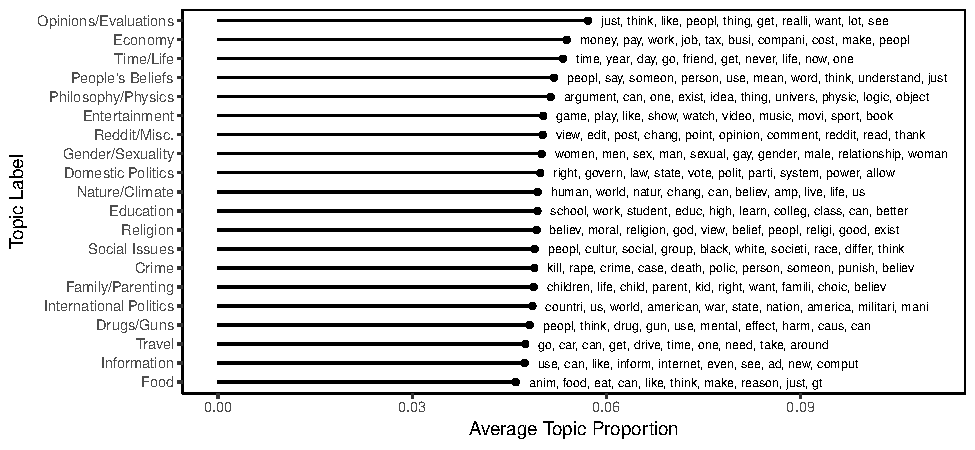
\includegraphics{/data/Dropbox/Uni/Projects/2017/cmv/calc/fig/topics.pdf}
\caption[Average topic proportions in opening statements on \texttt{/r/ChangeMyView/}]{Average topic proportions in opening statements on \texttt{/r/ChangeMyView/} based on a basic LDA model with 20 topics. The plot additionally displays the ten most likely terms associated with each respective topic.}\label{fig:lda}
\end{figure}

The Internet is not necessarily known as a place where people are willing to change their mind about \textit{any} issue. Yet, CMV maintains an open atmosphere that encourages users to acknowledge arguments that change their perspective. The rules of the subreddit state that users should ``Award a delta if you've acknowledged a change in your view. [...] Please note that a delta is not a sign of `defeat', it is just a token of appreciation towards a user who helped tweak or reshape your opinion. A delta also doesn't mean the discussion has ended.''\footnote{ \url{https://www.reddit.com/r/changemyview/wiki/rules}, last accessed April 22, 2018} Of course, this does not imply that every OP awards a $\Delta$ throughout a conversation. Figure~\ref{fig:delta} displays the number of discussion threads included in the dataset where OPs indicated that one of the responses changed their mind.

\begin{figure}[ht]
\centering
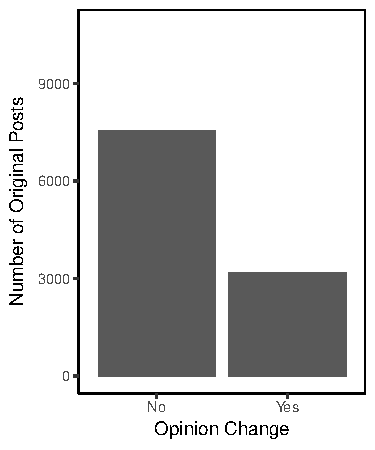
\includegraphics{/data/Dropbox/Uni/Projects/2017/cmv/calc/fig/delta.pdf}
\caption[Number of original posts on \texttt{/r/ChangeMyView/} that resulted in opinion change]{Number of discussions on \texttt{/r/ChangeMyView/} that resulted in opinion change (at least one $\Delta$ awarded by OP) versus not.}\label{fig:delta}
\end{figure}

In about two thirds of discussions on CMV between 2013 and 2015, OPs did not award a $\Delta$ for any of the counterarguments that were put forward, which leaves about 3,000 individual threads where OPs indicated that at least one of the responses changed their views. Interestingly, additional analyses included in the supplementary material show that there are only minimal differences in topic proportions between discussion threads that resulted in persuasion versus threads that did not (see Appendix~\ref{app:cmvstm}).

In their original study, \citet{tan2016winning} mainly investigated linguistic patterns (e.g., use of personal pronouns) and differences in style (formatting etc.) that predicted resistance to persuasion among OPs. They conclude for instance that ``comparative adjectives and adverbs are a sign of malleability, while superlative adjectives suggest stubbornness.'' The goal of the present analysis, in turn, is to go beyond linguistic patterns that are unrelated to content and explore the role of moral appeals in facilitating or inhibiting compromise. In order to capture moralized arguments, I rely on the MFT dictionary proposed by \citet{graham2009liberals}, which contains lists of word stems that signal each of the five moral foundations (care, fairness, loyalty, authority, sanctity) as well as a category of general moral terms.\footnote{See Appendix~\ref{app:cmvdict} for the complete dictionary.}

\begin{figure}[ht]
\centering
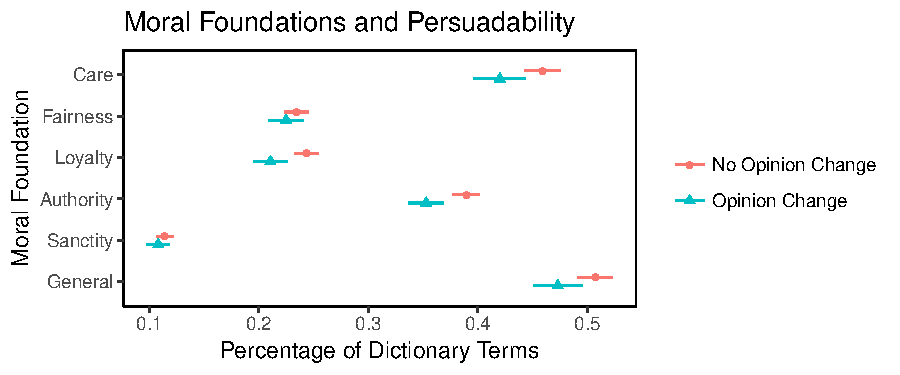
\includegraphics{/data/Dropbox/Uni/Projects/2017/cmv/calc/fig/persuadability.pdf}
\caption[Moral Foundations and Persuadability]{Moral Foundations and Persuadability: Average percentage of dictionary terms relative to the total number of words in each opening statement beginning a discussion, comparing discussions where the OP subsequently awarded a $\Delta$ (opinion change) or not (including 95\% confidence intervals).}\label{fig:persuadability}
\end{figure}

% ELABORATE ON CONSISTENCY WITH KRAFT ETC.
Figure~\ref{fig:persuadability} displays the percentage of dictionary terms for each foundation in the opening statements initiating a discussion on CMV (in proportion to the total number of words in each post). The plot compares the reliance on moral terms between OPs that subsequently changed their view versus OPs that did not. As an initial observation, it is interesting to note that the distribution of dictionary terms across foundations is strikingly similar to the proportions of moral terms in open-ended responses to the likes-dislikes questions included in the American National Election study \citep[c.f.,][]{kraft2018measuring}: The most prevalent dimensions are \textit{care} and \textit{authority}, while occurrences of \textit{sanctity} are largely negligible. Observing these similarities is noteworthy since they are suggestive of a common mechanism driving the emphasis on moral considerations when justifying preferences in a public opinion survey as well as in online discussions.

More important for the purposes of this paper is the fact that the percentage of dictionary terms across foundations appears smaller among opening statements that resulted in opinion change than among those that did not. More specifically, OPs who did not award any $\Delta$s in the subsequent discussion put a significantly stronger emphasis on moral considerations related to loyalty and authority ($p<.01$ in both cases after accounting for multiple comparisons using Bonferroni correction). Similar results can be obtained after aggregating all moral dictionary terms in a single category: OPs who were not persuadable on CMV use more words related to morality overall than OPs who indicate that the discussion changed their view ($p<.001$).

At first look, the findings appear consistent with the moral conviction literature, which posits that people who hold moralized attitudes are less willing to compromise and deviate from their prior beliefs \citep[e.g.,][]{skitka2005moral,ryan2014reconsidering,ryan2017no}. Yet, there are important issues that make it difficult to draw strong conclusions based on these initial results. First of all, there may be unobserved confounding factors that are related to both the OPs willingness to award $\Delta$s as well as the chosen discussion topic (which could be more or less aligned with moral considerations). The content of opening statements may also induce selection bias in user responses which can impact the nature of their comments and ultimately the productivity of discussions. Furthermore, there is no way of contrasting the potentially diverging impact of morally congruent arguments by exclusively examining the malleability of initial opinions. The following analyses address these problems by comparing the relative persuasiveness of arguments \textit{within a given discussion thread}.



\section{What Makes an Argument Persuasive?}
%\section{Determinants of Argument Persuasiveness}
% HOW DOES THIS RELATE TO THE SPECIFIC HYPOTHESES?

% SIGNPOST THAT I AM LOOKING FIRST AT THE OPENING STATEMENT, THEN REPLIES

The previous section demonstrated that the usage of moral terms in initial posts is predictive of the OPs' willingness to change their view in subsequent discussions. Now I focus directly on the persuasiveness of comments that are made in response to a given opening statement on CMV. In the context of the simplified discussion framework outlined above, I examine the arguments brought forward by $\mathcal{B}$, who is challenging $\mathcal{A}$'s view. This allows me to directly compare the moral conviction hypothesis with the moral foundations hypothesis, which have diverging predictions regarding the effectiveness of moralized appeals in discussions. Note that the arguments presented by $\mathcal{B}$ do not only include her initial post (i.e., the root response), but also any subsequent posts that are mentioned in the evolving discussion between $\mathcal{A}$ and $\mathcal{B}$ (i.e., the full response path).

In the original analysis by \citet{tan2016winning}, the authors implement a simple method to select pairs of arguments that respond to the same original post, with only one of the selected responses being successful in changing the OPs view. While differing in persuasiveness, arguments are matched in such a way that they are as similar as possible in terms of their word choice. More specifically, \citet{tan2016winning} select argument pairs by maximizing their Jaccard similarity:
\begin{equation}
\text{Jaccard}(B_\Delta,B_{\neg\Delta})=\dfrac{|B_\Delta\cap B_{\neg\Delta}|}{|B_\Delta\cup B_{\neg\Delta}|},
\end{equation}
where $B_\Delta$ and $B_{\neg\Delta}$ are the sets of words in two response paths associated with the same opening statement (one receiving a $\Delta$, the other not). In other words, they match each successful counterargument to an unsuccessful response that shares the largest proportion of common words (disregarding stopwords). As \citet[617]{tan2016winning} describe: ``This leads to a balanced binary prediction task: which of the two lexically similar rooted path-units is the successful one?''\footnote{As additional selection criteria and to avoid trivial posts, arguments are removed if they are shorter than 50 words, only include clarifying questions, or if the opening statement received fewer than 10 responses overall and fewer than 3 unsuccessful challenges \citep[see][617 for details]{tan2016winning}.}

The analyses reported below rely on this approach to select matched argument pairs for comparison. To reiterate, I focus on discussions in which OPs awarded at least one $\Delta$. The response that received a $\Delta$ is then matched to another counterargument that was not successful in changing  the OPs view but is as similar as possible in terms of its vocabulary. Note that in principle, this strategy should make it more difficult to find differences in the MFT dictionaries as argument pairs are matched based on their lexical similarity. One might worry, however, that the necessary initial selection on discussions where OPs ultimately awarded at least one $\Delta$ might disproportionately discard cases where the initial statement emphasized moral considerations. Luckily, that is not the case. Figure~\ref{fig:mft_op_all} shows that almost all of the opening statements in the matched pair selection mention at least one of the moral dictionary terms. Furthermore, the proportion of moral dictionary terms among this set of opening statement shows the same pattern as in Figure~\ref{fig:persuadability} (results included in Appendix~\ref{app:paired}).

\begin{figure}[ht]
\centering
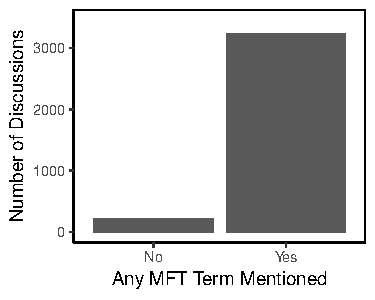
\includegraphics{/data/Dropbox/Uni/Projects/2017/cmv/calc/fig/mft_op_all.pdf}
\caption[Number of opening statements in the paired argument data that included \textit{any} term mentioned in the MFT dictionary]{Number of opening statements in the paired argument data that included \textit{any} term mentioned in the MFT dictionary.}\label{fig:mft_op_all}
\end{figure}

An important issue that remains unresolved using this approach is that the matching procedure only focuses on the set of unique words that are used in each response path and does not take into account their relative length. This can be especially problematic since persuasive discussions tend to be longer and involve at least a few back-and-forth exchanges between the OP and the challenger \citep[c.f.,][616]{tan2016winning}. Figure~\ref{fig:wordcount_violin} displays the distribution of the differences in word counts between successful and unsuccessful argument pairs. Clearly, longer responses are more likely to be awarded a $\Delta$, which might jeopardize potential inferences about the relative reliance on moral dictionary terms.

\begin{figure}[ht]
\centering
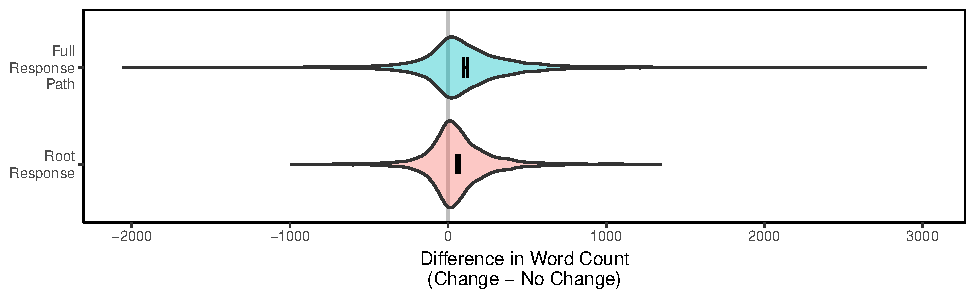
\includegraphics{/data/Dropbox/Uni/Projects/2017/cmv/calc/fig/wordcount_violin.pdf}
\caption[Difference in response lengths between successful and unsuccessful counterarguments]{Difference in response lengths between successful and unsuccessful counterarguments. The narrow black bars display the 95\% confidence interval of mean differences.}\label{fig:wordcount_violin}
\end{figure}

As a first step to alleviate this concern, it is worth noting that I only examine the \textit{percentages} of MFT dictionary occurrences in each discussion rather than a raw count, which implies that the prevalence of moral considerations is standardized by the overall length of each post. Notwithstanding, I take additional precautions proposed by \citet{tan2016winning} to check the robustness of the results. First, I not only examine differences when looking at the entire response path of a discussion between two users (i.e., all posts that were part of the dialogue with the OP), but restrict the analysis to focus on the challenger's root response to the opening statement only. As can be seen in Figure~\ref{fig:wordcount_violin}, the differences in word counts between argument pairs are significantly smaller. Recovering the same patterns in the root response as in the full response path implies that the initial arguments that triggered an exchange with the OP are by themselves predictive of the outcome of the discussion. To be fair, there are still substantial differences in the length of successful versus unsuccessful root responses. As a second robustness check, I additionally truncate the longer root response of a given pair as follows: I count the total number of words in each post and simply cut off the end of the longer response such that both word counts in a given pair are exactly equal. Using this framework, I now turn to the analysis of the persuasiveness of moral arguments made in discussions on CMV.


\subsection{Moral Appeals are Futile...}
%\subsection{Appeals to Morality are Futile...}
%\subsection{Moral Appeals and Opinion Change}

Recall that the moral conviction hypothesis posits that arguments that involve moral appeals will be less persuasive than arguments that do not involve moral appeals. In order to test this proposition, I examine the matched argument pairs within discussions and compare MFT dictionary term proportions between contributions that were successful in receiving a $\Delta$ and those that were unsuccessful. Figure~\ref{fig:persuasiveness} displays the respective differences between matched argument pairs. Positive values indicate that arguments that received a $\Delta$ contained a larger percentage of dictionary terms, and vice versa. Again, according to the literature on moral conviction, we would expect the opposite, namely that persuasive arguments should focus less on moral considerations. As discussed previously, the analyses are implemented for the full response path as well as focusing only on (truncated) root responses.

\begin{figure}[ht]
\centering
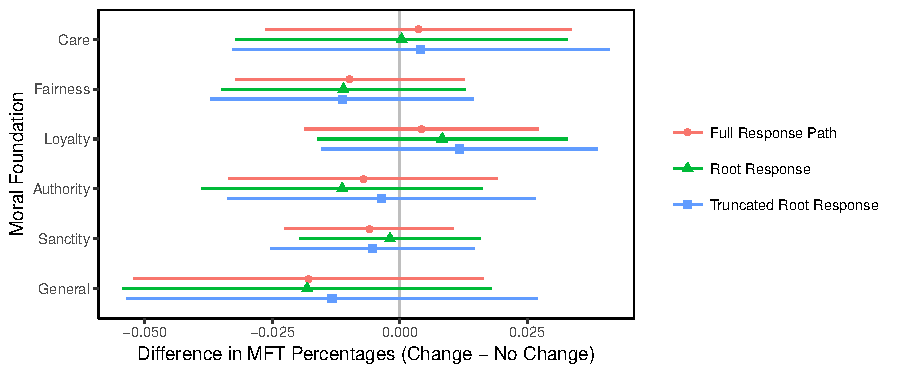
\includegraphics{/data/Dropbox/Uni/Projects/2017/cmv/calc/fig/persuasiveness.pdf}
\caption[Moral Foundations and Persuasiveness]{Moral Foundations and Persuasiveness: Average difference of dictionary term percentages relative to the total number of words in each post, comparing counterarguments where the OP subsequently awarded a $\Delta$ (opinion change) or not (including 95\% confidence intervals).}\label{fig:persuasiveness}
\end{figure}

The results show that evoking moral considerations in counterarguments does not affect the likelihood of changing the OPs' view on a given issue. This finding furthermore holds after combining all moral terms in an aggregate dictionary and comparing matched proportions between argument pairs ($p > .34$). Moralized arguments as such are therefore no less persuasive and do not decrease the likelihood of compromise, a result that is not consistent with the moral conviction literature.



\subsection{...Unless We're Speaking the Same Moral Language}

In contrast to the moral conviction hypothesis, moral foundations theory suggests that we cannot fully understand the effect of moral appeals without taking into account the discussion partner's moral framework.  What is decisive from this perspective is the congruence in moral arguments between both discussants. I measure the moral congruence between an OP's opening statement and each counterargument by computing the cosine similarity in their respective MFT dictionary scores. In general, using cosine similarities based on vectors of word counts is a standard approach in text analysis to quantify the similarity of documents independent of their length \citep[e.g.,][]{manning2008introduction}. More formally, moral congruence can therefore be written as:
\begin{equation}
\text{MFT Congruence}=\dfrac{\vec{a}\cdot \vec{b}}{||\vec{a}||\hspace{.2em}||\vec{b}||},
\end{equation}
where $\vec{a}$ is the vector of dictionary counts in the OP's opening statement and $\vec{b}$ is the respective vector for a response. The measure ranges from 0 (no moral overlap) to 1 (equal emphasis on the same moral foundations). Moral congruence is also set to zero if either one of the statements does not contain a single term included in the dictionary.

To reiterate, the moral foundations hypothesis posits that arguments that involve moral appeals will be more persuasive than arguments that do not involve moral appeals, but only if they are congruent with the opening statement's moral framework. In contrast, the moral conviction literature would predict a negative effect of moral congruence, since it implies that both discussants, who hold opposing views on an issue, use moralized arguments that ultimately reduce the potential for compromise.

Figure~\ref{fig:cosine} displays the difference in moral congruence between successful and unsuccessful arguments. Positive values indicate that posts that were ultimately awarded a $\Delta$ by the OP used moral appeals that had a higher congruence with the OP's opening statement. The results clearly show that consistent with MFT, moral congruence is larger in persuasive than in non-persuasive arguments.

\begin{figure}[ht]
\centering
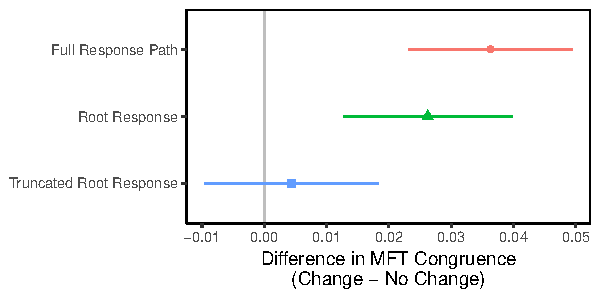
\includegraphics{/data/Dropbox/Uni/Projects/2017/cmv/calc/fig/cosine.pdf}
\caption[Moral congruence and persuasiveness]{Moral congruence and persuasiveness: Average differences between successful and unsuccessful counterarguments in cosine similarities with the opening statements (including 95\% confidence intervals).}\label{fig:cosine}
\end{figure}

The positive relationship between moral congruence and persuasiveness remains significant irrespective of whether I examine the content of the entire discussion (full response path), or restrict the analysis to each user's first post challenging the OP (root response). However, the mean difference in moral congruence does not reach conventional levels of statistical significance after truncating root responses to the same length for each pair. This finding could either suggest that the truncation procedure introduces too much noise to recover any differences, or alternatively that the measure of moral congruence is confounded by the differential length of successful and unsuccessful posts. The former seems less likely to be an issue because I recovered only marginal differences in raw dictionary term percentages between raw and truncated rooted responses in the previous section.

It is also important to emphasize that the higher moral congruence among persuasive posts is by no means driven by the fact that successful arguments use similar language to the opening statement \textit{in general}. Quite contrary, \citet[618]{tan2016winning} concluded in their study that when looking at the entire vocabulary of responses (excluding stopwords),  then persuasive arguments used significantly more \textit{different wording} than original post. In other words, a similar general vocabulary across all words is less persuasive, whereas a similar use of terms belonging to each moral foundation proved to be more persuasive. As such, the results presented here appear to capture the unique persuasive effect of morally congruent arguments.



% ADD EXAMPLE FROM DATA IN THE END!!!
% How strong are these differences in moral congruence? Do we actually capture meaningful variation? It turns out that the example of CMV discussions intially presented were selected based on the fact that the successful.



\section{Conclusion}\label{conclusion}

Political elites on both sides of the aisle routinely rely on moral rhetoric in order to bolster their views, which induces strong emotional reactions among citizens \citep{lipsitz2017playing} and can ultimately influence their attitudes \citep[e.g.,][]{clifford2013words,clifford2015concerns}. As such, it does not seem surprising that the increasingly partisan and polarized environment in the United States has been linked to stronger tendencies among citizens to moralize politics \citep{garrett2018moral}. Is the only solution to overcome this trend to de-emphasize moral convictions when discussing political issues? Or is it rather the case that morality may even be helpful in overcoming disagreements as long as people rely on the same moral frameworks?

The present paper addresses these questions by contrasting two strands of research in moral psychology that lead to diverging predictions regarding the role of morality in political compromise. Previous work on moral conviction suggests that individuals who moralize politics should be less willing to compromise and therefore resist persuasion through moral appeals. On the other hand, moral foundations theory posits that compromise is indeed possible as long as the discussants use the same moral language.

Both competing hypotheses are tested by relying on a unique dataset of online discussions on the Reddit community CMV compiled by \cite{tan2016winning}. Overall, the empirical patterns support moral foundations theory and stand in contrast to predictions rooted in the literature on moral conviction. While general levels of moralization have little impact on argument persuasiveness, the results show that an argument's moral congruence with the discussant's opening statement increases the likelihood of changing his or her view. As such, moral appeals can facilitate compromise and change people's minds as long as they are consistent with their existing moral frameworks. Rather than automatically driving people further apart, moral appeals might therefore help bridge the growing divide between liberals and conservatives. More broadly, the paper shows that the field of moral psychology stands to benefit from a further integration of two prominent theoretical frameworks that developed largely independent of each other and---unfortunately---still exhibit relatively little interconnections.

At the same time, the analysis presented here has important limitations. One of the biggest potential issues is the fact that the matched argument pairs differ in length, which may confound the relationship between morality and persuasiveness. I addressed this concern by only examining measures that are standardized by the total number of words in each post and by examining root responses in addition to full response paths. The results are largely robust to these varying specifications, with the important exception of the effect of moral congruence in the truncated root response. More generally, while it is a substantial advantage that the discussions on CMV cover a wide range of topics, it can be argued that some of them are ultimately irrelevant for moral considerations (such as software and technology).\footnote{For example, users discussed their preferences for the Windows operating system as compared to macOS X, which is obviously fruitless since Linux is superior to either of them and anyone who says otherwise is wrong.} On the other hand, such inherently non-political and non-moral discussions should not induce any systematic biases between successful and non-successful arguments. For the purpose of this paper, I decided against filtering out subsets of discussions based on their thematic relevance. Even though such a strategy may arguably reduce measurement error, it introduces potential selection bias at the same time. I leave it to future research to leverage more controlled environments and focus on specific (political) issues---for example in the context of laboratory experiments. In contrast to framing studies conducted in the past, however, it is time to open the black box of conversations and directly examine the content of discussions in order to better understand the mechanisms underlying attitude change, persuasion, and compromise.



% TALK about potential limitations: selection bias, etc.

% TO DOs, future directions, etc.:
% - examine specific topics (e.g., climate change etc.)[ ]
% - clean original posts (links etc)[x]
% - adjust confidence intervals to correct for multiple comparisons [x]
% - improve code documentation, add comments in internal functions [ ]
% - check MFT scores in argument pairs (as well as OP entry) [x]
% - take into account clustering in paired data! OPs appear multiple times [ ]
